\documentclass[a4paper, 12pt]{article}
\usepackage[a4paper,top=1.5cm, bottom=1.5cm, left=1cm, right=1cm]{geometry}

% Работа с русским языком
\usepackage[utf8]{inputenc}
\usepackage{mathtext}                % русские буквы в формулах
\usepackage[english, russian]{babel} % локализация и переносы

\usepackage{graphicx}   % Вставка изображений
\usepackage{float}      % "Плавающие" изображения3
\usepackage{wrapfig}    % Обтекание фигур (таблиц, картинок и прочего)
\usepackage{subfig}
\graphicspath{ {./images/} }

\usepackage{tabularx}
\usepackage{multirow}
\usepackage{booktabs}
\usepackage{amsmath}
\usepackage{amsfonts}
\usepackage{indentfirst}
\usepackage{longtable}
\usepackage{natbib}
\usepackage{bm}

\newcommand{\elem}[3]{{}^{#2}_{#3}\text{#1}}
\newcommand{\Cs}{\elem{Cs}{137}{}}

%%% Колонтитулы
\usepackage{titleps}
\newpagestyle{main}{
	\setheadrule{0.4pt}
	\sethead{Отчёт о выполнении лабораторной работы 4.2}{}{}
	\setfootrule{0.4pt}                       
	\setfoot{ФРКТ МФТИ, 2024}{}{\thepage} 
}
\pagestyle{main}  

\begin{document}
    \begin{titlepage}
	\begin{center}
            {\large МОСКОВСКИЙ ФИЗИКО-ТЕХНИЧЕСКИЙ ИНСТИТУТ (НАЦИОНАЛЬНЫЙ ИССЛЕДОВАТЕЛЬСКИЙ УНИВЕРСИТЕТ)}
	\end{center}
 
	\begin{center}
		{\large Физтех-школа радиотехники и компьютерных технологий}
	\end{center}
	
	\vspace{8cm}
	{\LARGE
		\begin{center}
                {\bf Отчёт о выполнении лабораторной работы 4.2}\\
                Исследование энергетического спектра $\beta$-частиц и определение их максимальной энергии при помощи магнитного спектрометра
		\end{center}
	}
	\vspace{3 cm}
	\begin{flushright}
		{\Large Авторы: \\ 
        Тихонов Дмитрий Романович, \\ студент группы Б01-206а \\
        Павловский Кирилл Михайлович, \\ студент группы Б01-206а}
	\end{flushright}
	\vspace{4cm}
	\begin{center}
		\Large Долгопрудный, 2024
	\end{center}
    \end{titlepage}


    \section{Введение}

    \noindent \textbf{Цель работы:} исследовать энергетический спектр $\beta$-частиц при распаде ядер $\Cs$ и определить их максимальную энергию. \\
	
    \noindent \textbf{В работе используются:} магнитный спектрометр с <<короткой линзой>>, форвакуумный насос и вакууметр, персональный ЭВМ, высоковольтный и низковольтный выпрямители.
    
    \section{Теоретическое введение}

    \textit{Бета-распадом} называется самопроизвольное превращение ядер, при котором их массовое число не изменяется, а заряд увеличивается или уменьшается на единицу. Бета-активные ядра встречаются во всей области значений массового числа $A$, начиная от единицы (свободный нейтрон) и кончая самыми тяжелыми ядрами. Период полураспада $\beta$-активных ядер изменяется от ничтожных долей секунды до $10^{18}$ лет. Выделяющаяся при единичном акте $\beta$-распада энергия варьируется от 18 кэВ до 13,4 МэВ.

    В данной работе мы будем иметь дело с электронным распадом

    \begin{equation*}
        ^A_ZX \rightarrow ^{\; \; \; \; \: A}_{Z+1}X + e^- + \widetilde{\nu},
    \end{equation*}

    при котором кроме электрона испускается антинейтрино. Освобождающаяся при $\beta$-распаде энергия делится между электроном, антинейтрино и дочерним ядром, однако доля энергии, передаваемой ядру, исчезающе мала по сравнению с энергией, уносимой электроном и антинейтрино. Практически можно считать, что эти две частицы делят между собой всю освобождающуюся энергию. Поэтому электроны могут иметь любое значение энергии  от нулевой до некоторой максимальной, которая равна энергии, освобождающейся при $\beta$-распаде, являющейся важной физической величиной.

    Вероятность $dw$ того, что при распаде электрон вылетит с импульсом в интервале $d^3\mathbf{p}$, а антинейтрино с импульсом в интервале $d^3\mathbf{k}$, пропорциональна произведению этих дифференциалов. Но мы должны еще учесть закон сохранения энергии, согласно которому импульсы $\mathbf{p}$ и $\mathbf{k}$ электрона и антинейтрино связаны соотношением

    \begin{equation}
        E_e - E - ck = 0,
    \end{equation}

    где $E_e$ - максимальная энергия электрона, кинетическая энергия электрона $E$ связана с его импульсом обычным релятивистским соотношением

    \begin{equation}
        E = c\sqrt{p^2 + m^2c^2} - mc^2,
    \end{equation}

    а через $ck$ обозначена энергия антинейтрино с импульсом $k$. Условие можно учесть введением в выражение для $dw$ $\delta$-функции
    \begin{equation}
        \delta (E_e - E - ck).
    \end{equation}

    Таким образом, вероятность $dw$ может быть записана в виде

    \begin{equation}
        \label{eq:dw}
        dw = D \delta (E_e - E - ck)d^3 \mathbf{p} d^3 \mathbf{k} = D \delta (E_e - E - ck)p^2dpk^2dkd{\Omega}_ed{\Omega}_{\widetilde{\nu}},
    \end{equation}

    где $D$ -- некоторый коэффициент пропорциональности, $d\Omega_e$ , $d\Omega_{\widetilde{\nu}}$ -- элементы телесных углов направлений вылета электрона и нейтрино. Вероятность $dw$ непосредственно связана с $\beta$-спектром, поскольку для большого числа $N_0$ распадов число $dN$ распадов с вылетом электрона и антинейтрино с импульсом соответственно от $\mathbf{p}$ до $\mathbf{p} + d\mathbf{p}$ и от $\mathbf{k}$ до $\mathbf{k} + d\mathbf{k}$ определяется соотношением

    \begin{equation}
        \label{eq:dN(dw)}
        dN = N_0 dw.
    \end{equation}

    Коэффициент $D$ в формуле \eqref{eq:dw} можно считать для рассматриваемых нами так называемых разрешенных фермиевских типов распадов с хорошей точностью константой (разрешенными называются такие переходы, при которых не изменяются ни момент, ни четность состояния ядра). В этом случае величину $dw$ из \eqref{eq:dN(dw)} можно проинтегрировать по всем углам и по абсолютному значению импульса нейтрино.

    После умножения на полное число распадов $N_0$ проинтегрированное выражение приобретает смысл числа электронов $dN$, вылетающих из ядра с импульсом, абсолютная величина которого лежит между $p$ и $ p + dp$:

    \begin{equation}
        \label{eq:dN}
        dN = \dfrac{16\pi^2 N_0}{c^2}Dp^2(E_e - E)^2dp.
    \end{equation}

    Чтобы получить распределение электронов по энергиям, надо в \eqref{eq:dN} перейти от $dp$ к $dE$:

    \begin{equation}
        dE = \dfrac{c^2p}{E + mc^2}dp,
    \end{equation}

    после чего выражающая форму $\beta$-спектра величина $N(E) = dN/dE$ приобретает вид

    \begin{equation}
        \label{eq:dN/dE}
        \dfrac{dN}{dE} = N_0Bcp(E + mc^2)(E_e - E)^2 = N_0B\sqrt{E(E + 2mc^2)}(E_e - E)^2(E + mc^2)
    \end{equation}

    где $B = (16\pi^2/c^4)D$. В нерелятивистском приближении, которое и имеет место в нашем случае, выражение \eqref{eq:dN/dE} упрощается, и мы имеем

    \begin{equation}
        \label{eq:dN/dE_approx}
        \dfrac{dN}{dE} \approx \sqrt{E}(E_e - E)^2.
    \end{equation}

    \begin{figure}[H]
        \centering
        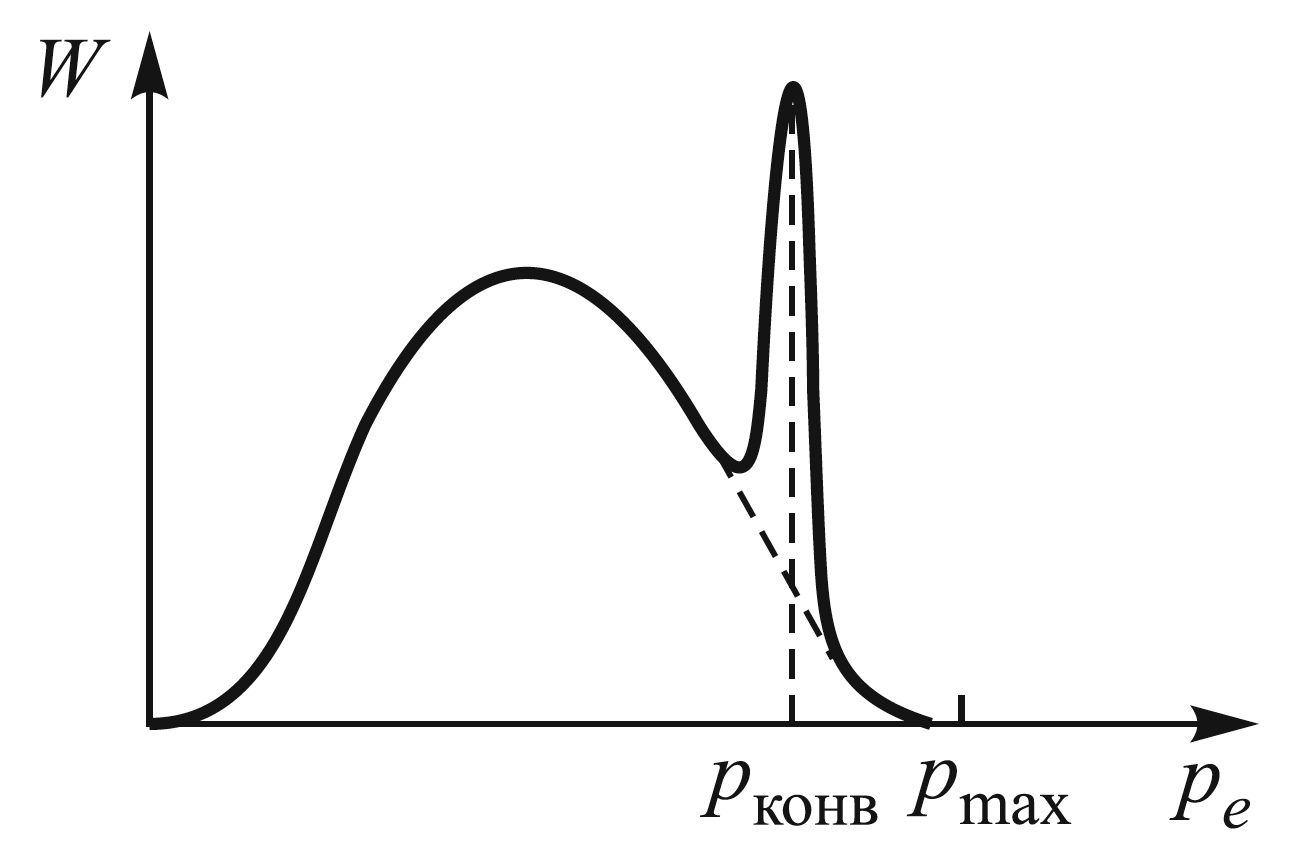
\includegraphics[width = 0.5\linewidth]{images/spectrum_th.jpg}
        \caption{Форма спектра $\beta$-частиц при разрешенных переходах}
        \label{fig:spectrum_th}
    \end{figure}

    Выражение \eqref{eq:dN/dE_approx} приводит к спектру, имеющему вид широкого колокола (рис.\ref{fig:spectrum_th}). Кривая плавно отходит от нуля и столь же плавно, по параболе, касается оси абсцисс в области максимальной энергии электронов $E_e$. 

    Дочерние ядра, возникающие в результате $\beta$-распада, нередко оказываются возбужденными. Возбужденные ядра отдают свою энергию либо излучая $\gamma$-квант (энергия которого равна разности энергий начального и конечного уровней), либо передавая избыток энергии одному из электронов с внутренних оболочек атома. Излучаемые в таком процессе электроны имеют строго определенную энергию и называются \textit{конверсионными}.

    Конверсия чаще всего происходит на оболочках $K$ или $L$. На спектре, представленном на рис. \ref{fig:spectrum_th}, видна монохроматическая линия, вызванная электронами конверсии. Ширина этой линии в нашем случае является чисто аппаратурной -- по ней можно оценить разрешающую силу спектрометра.
    
    \newpage
    
    \section{Методика измерений и экспериментальная установка}

    Для определения энергии $\beta$-частиц в работе используется магнитный спектрометр, схема которого показана на рисунке \ref{fig:installation}. 

    \begin{figure}[H]
        \centering
        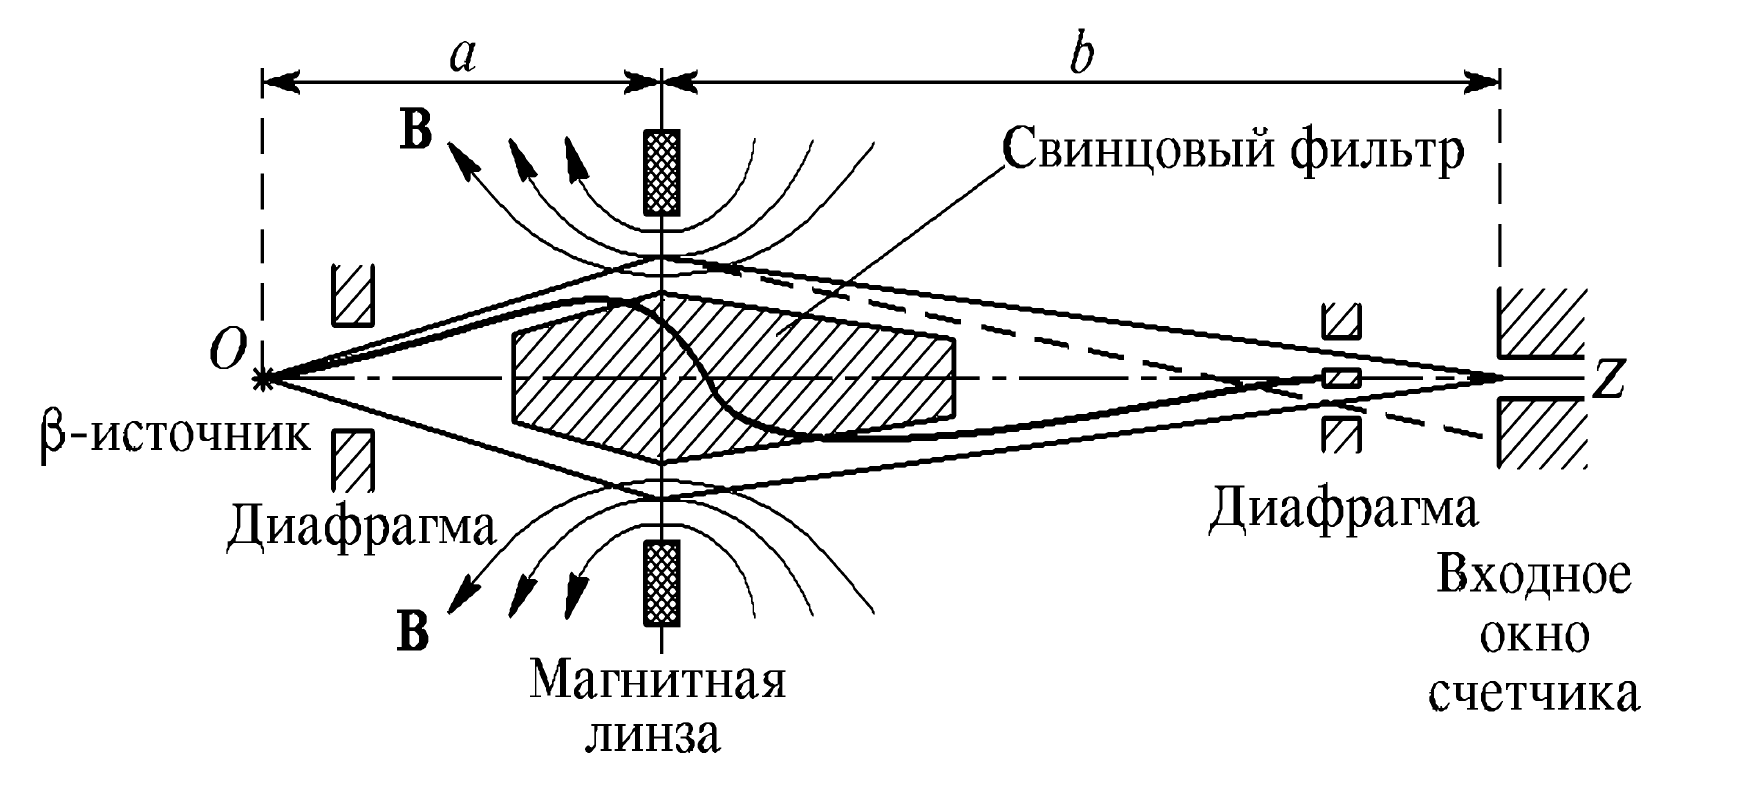
\includegraphics[width = 0.5\linewidth]{images/installation.png}
        \caption{Схема $\beta$-спектрометра с короткой магнитной линзой}
        \label{fig:installation}
    \end{figure}
    
    Электроны испускаются радиоактивным источником и попадают в магнитное поле катушки, ось которой параллельна $OZ$. Траектории электронов сходятся в одной точке -- фокусе, где и установлен сцинтилляционный счетчик, сигналы которого усиливаются фотоумножителем и регистрируются пересчетным прибором. Фокусное расстояние $f$ магнитной линзы связано с током в катушке $I$ и импульсом $p_e$ регистрируемых частиц следующим образом:

    \begin{equation}
        \frac{1}{f} \propto \frac{I^2}{p_e^2}
    \end{equation}
		
    При неизменной геометрии установки, увеличивая и уменьшая силу тока, можно фокусировать электроны разных импульсов, причем 
	
    \begin{equation}
        \label{eq:pkI}
        p_e = kI,
    \end{equation}
	
    где $k$ --- коэффициент пропорциональности, являющийся параметром установки.

    В $\beta$-спектрометре установлены диафрагмы для ограничения углов вылета частиц из источника и свинцовый фильтр для защиты от прямого попадания $\gamma$-лучей. 

    Число частиц $N$, регистрируемых на установке, равно $N \approx W(p_e) \cdot \Delta p_e$, где $\Delta p_e$ - разрешающая способность спектрометра. Дифференцируя выражение для фокуса магнитной линзы, получим: $\Delta p_e = \frac{1}{2}\frac{\Delta f}{f}p_e$, то есть $\Delta p_e \propto p_e$. Таким образом, для количества частиц справедлива формула: 

    \begin{equation}
        \label{eq:N}
        N = CW(p_e)p_e,
    \end{equation}

    где $C$ - некоторая константа.

    \begin{figure}[H]
        \centering
        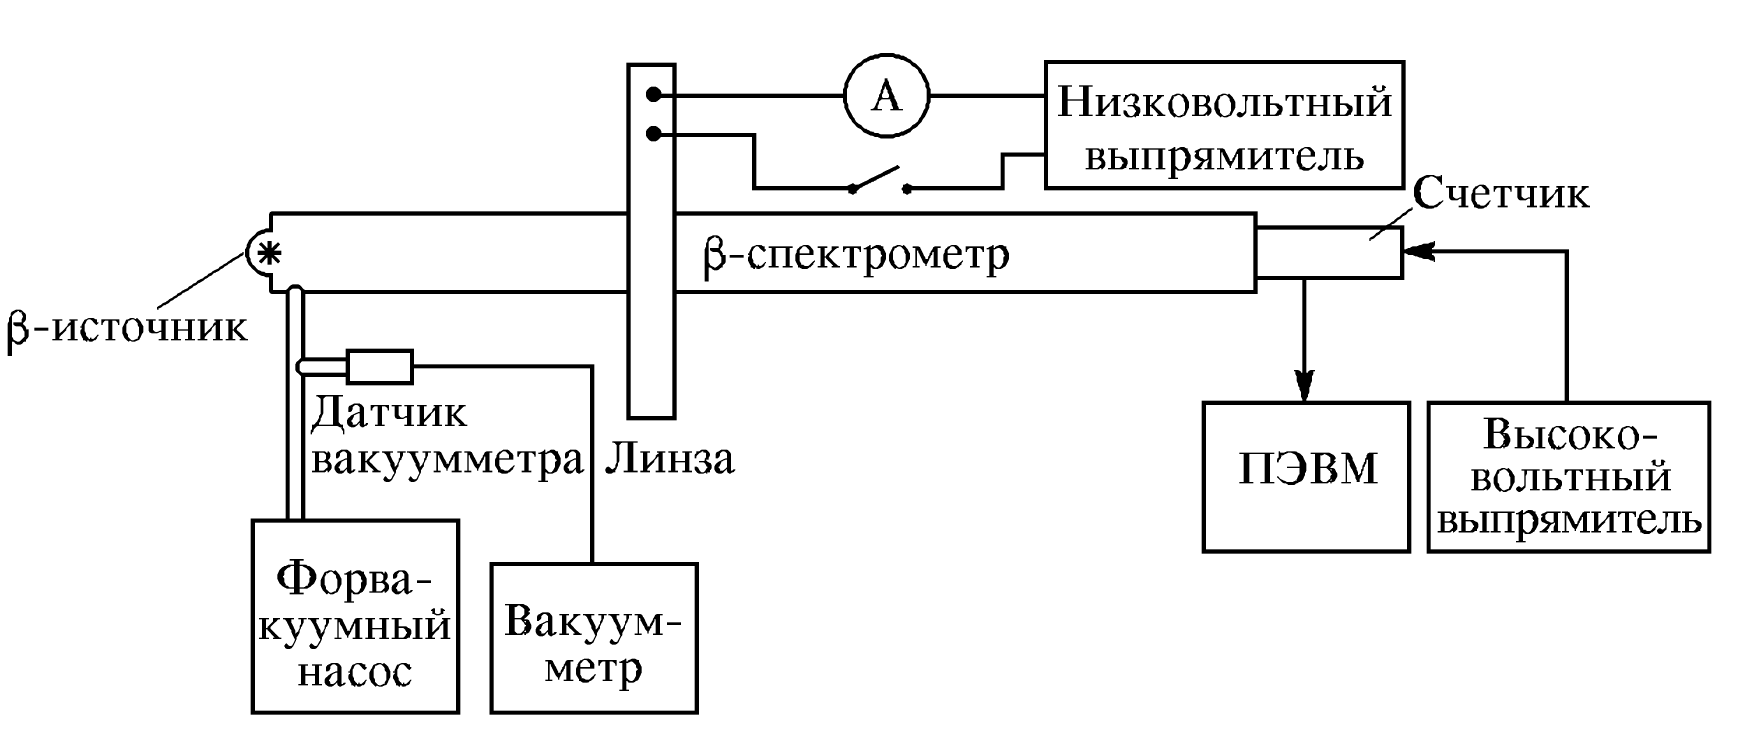
\includegraphics[width = 0.5\linewidth]{images/scheme.png}
        \caption{Блок-схема установки для изучения $\beta$-спектра}
        \label{fig:scheme}
    \end{figure}

    \newpage
	
    \section{Результаты измерений и обработка данных}

    На рис. \ref{fig:spectrum} приведён cпектр $\beta$-распада атома $^{137}$Cs. 

    \begin{figure}[H]
        \centering
        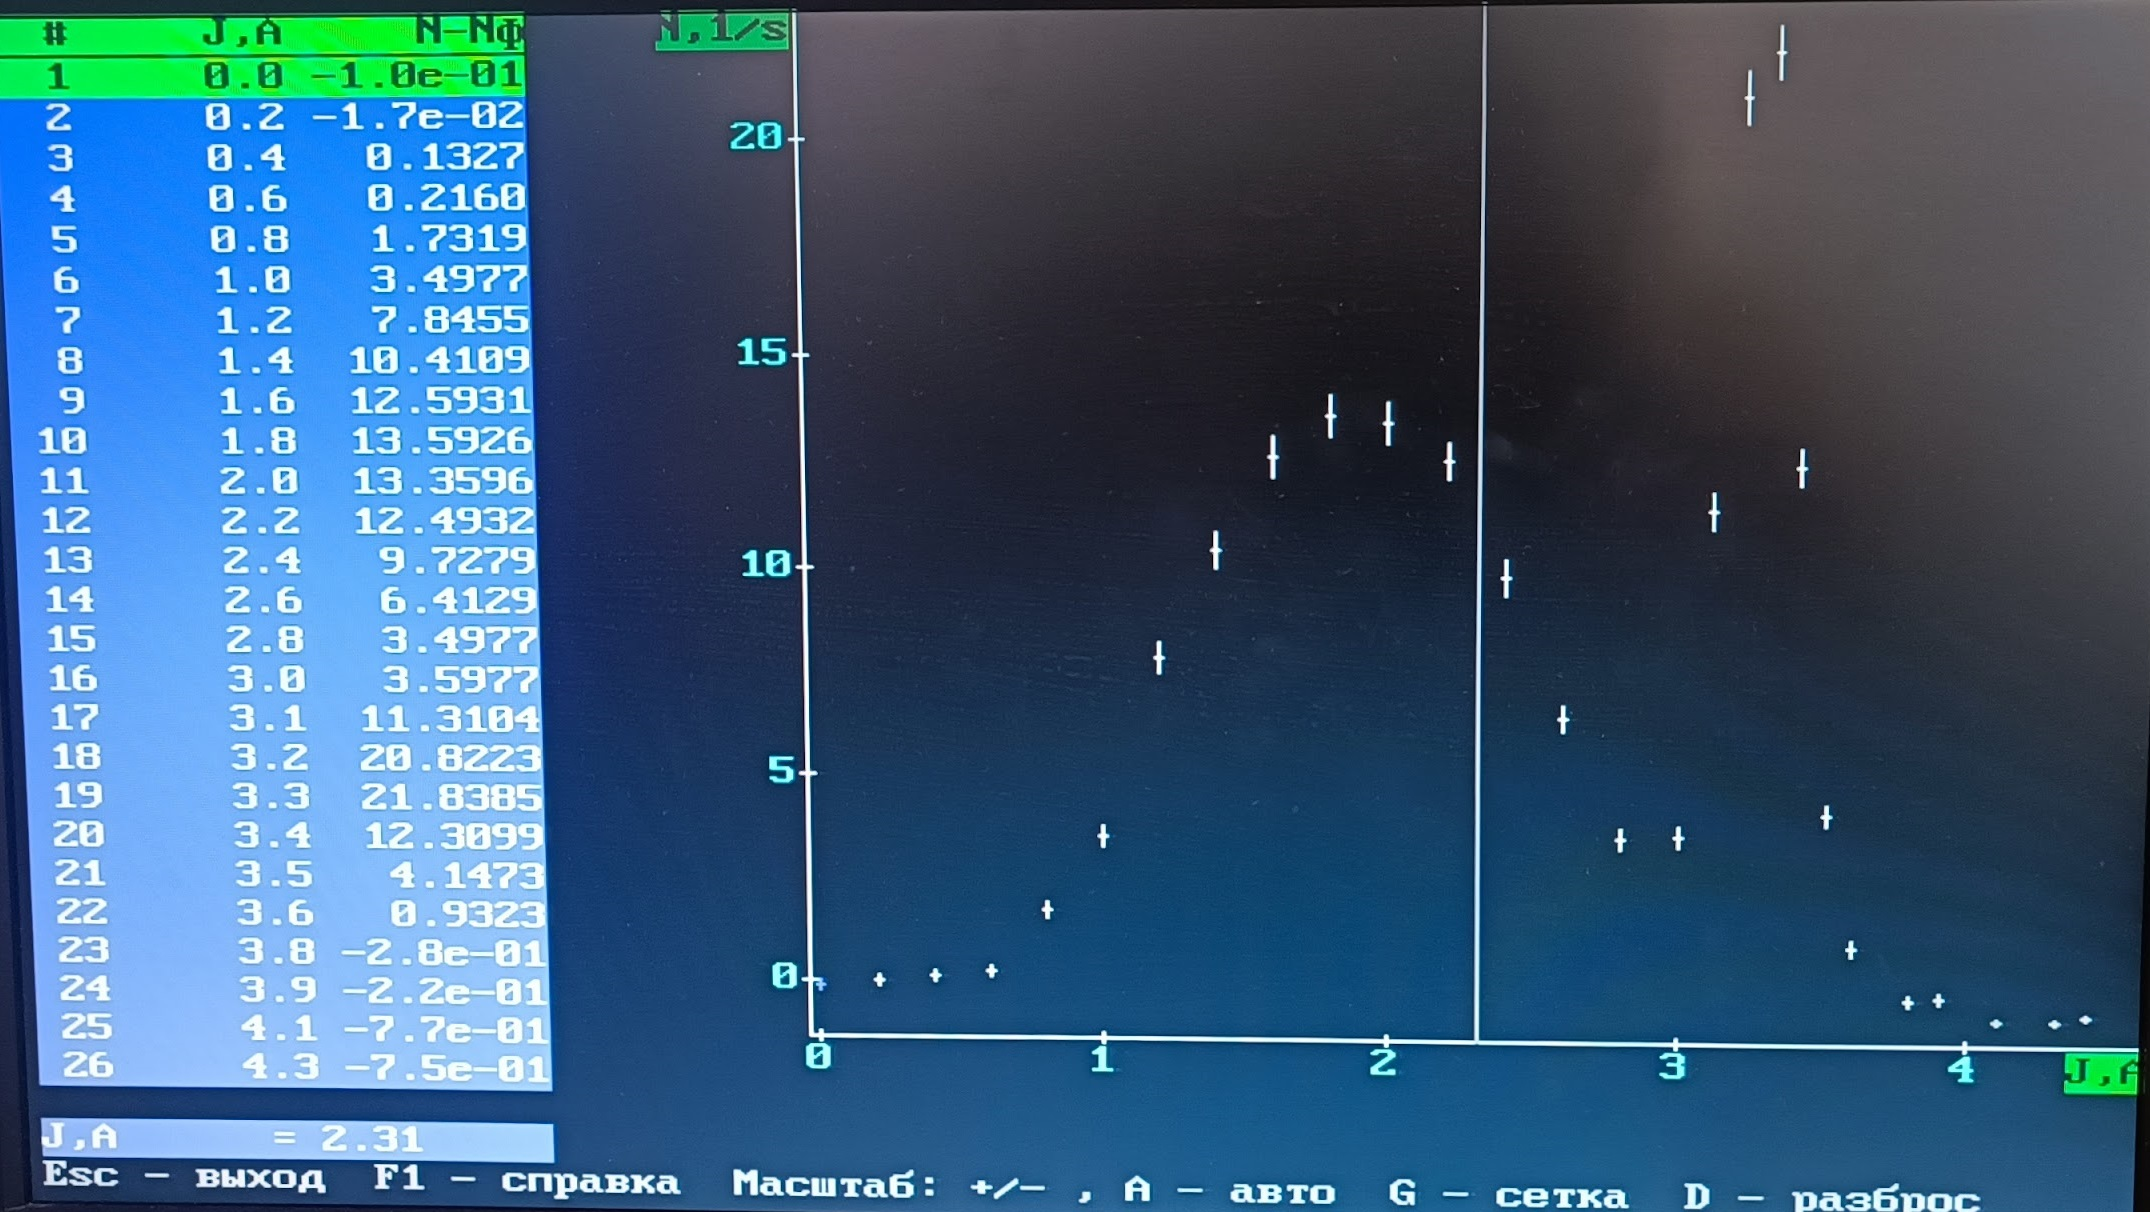
\includegraphics[width=0.5\linewidth]{images/spectrum.jpg}
        \caption{Спектр $\beta$-распада атома $\Cs$}
        \label{fig:spectrum}
    \end{figure}
    
    Откалибруем его. Для этого с помощью встроенной в ЭВМ программы пересчитаем значения силы тока в импульс по формуле (\ref{eq:pkI}). Коэффициент $k$ определим по известной конверсионной линии:
    
    $$1013.5 \ \text{кэВ} = kcI_0,$$
    
    где $c$ -- скорость света, $I_0 = 3.25$ А -- сила тока, при которой наблюдается конверсионный пик.
		
    Сдвиг графика по оси ординат сделаем на величину радиационного фона $N_\text{ф}$.

    \begin{figure}[H]
        \centering
        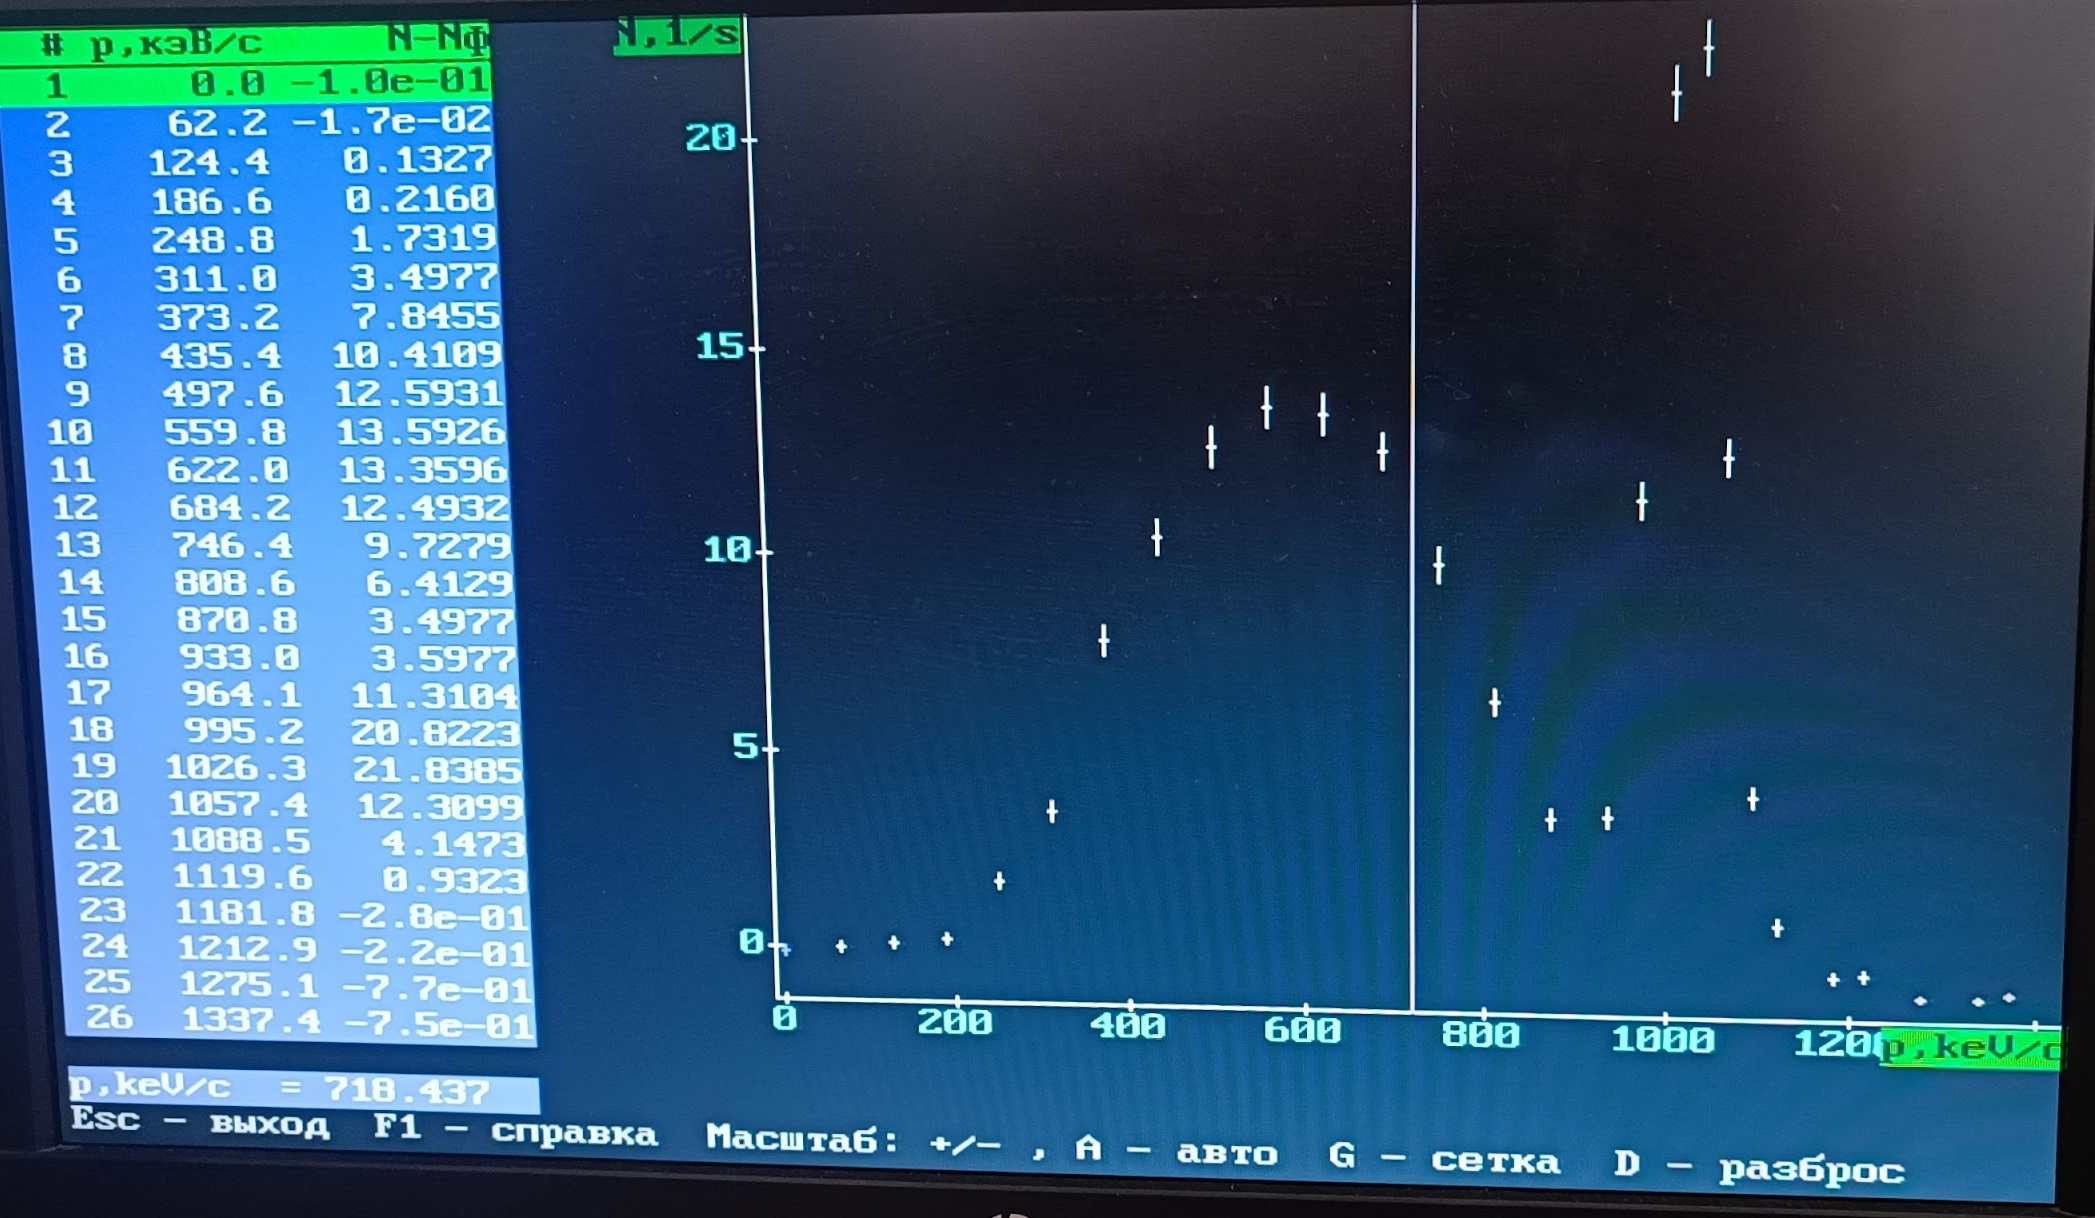
\includegraphics[width=0.5\linewidth]{images/calibrated_spectrum.jpg}
        \caption{Откалиброванный спектр $\beta$-распада атома $\Cs$}
        \label{fig:calibrated_spectrum}
    \end{figure}
		 
    Определим максимальную энергию $\beta$-спектра. Анализ рис.~\ref{fig:calibrated_spectrum} в таком случае даст достаточно грубый результат, так как нам придётся ограничиться исследованием точек у самой верхней границы спектра. Эти точки измерены с наименьшей статистической точностью. Можно уменьшить ошибку определения максимальной энергии посредством процедуры Ферми-Кюри. Для этого мы отложим по оси ординат величину $\sqrt{N}/p^{3/2}$, а по оси абсцисс энергию $\beta$-частиц (с учётом того, что энергия электронов внутренней конверсии $^{137}$Cs равна 634 кэВ). В таком случае мы задействуем большинство экспериментальных точек, и прежде всего точки середины $\beta$-спектра, которые измерены с наилучшей точностью.

    \begin{figure}[H]
        \centering
        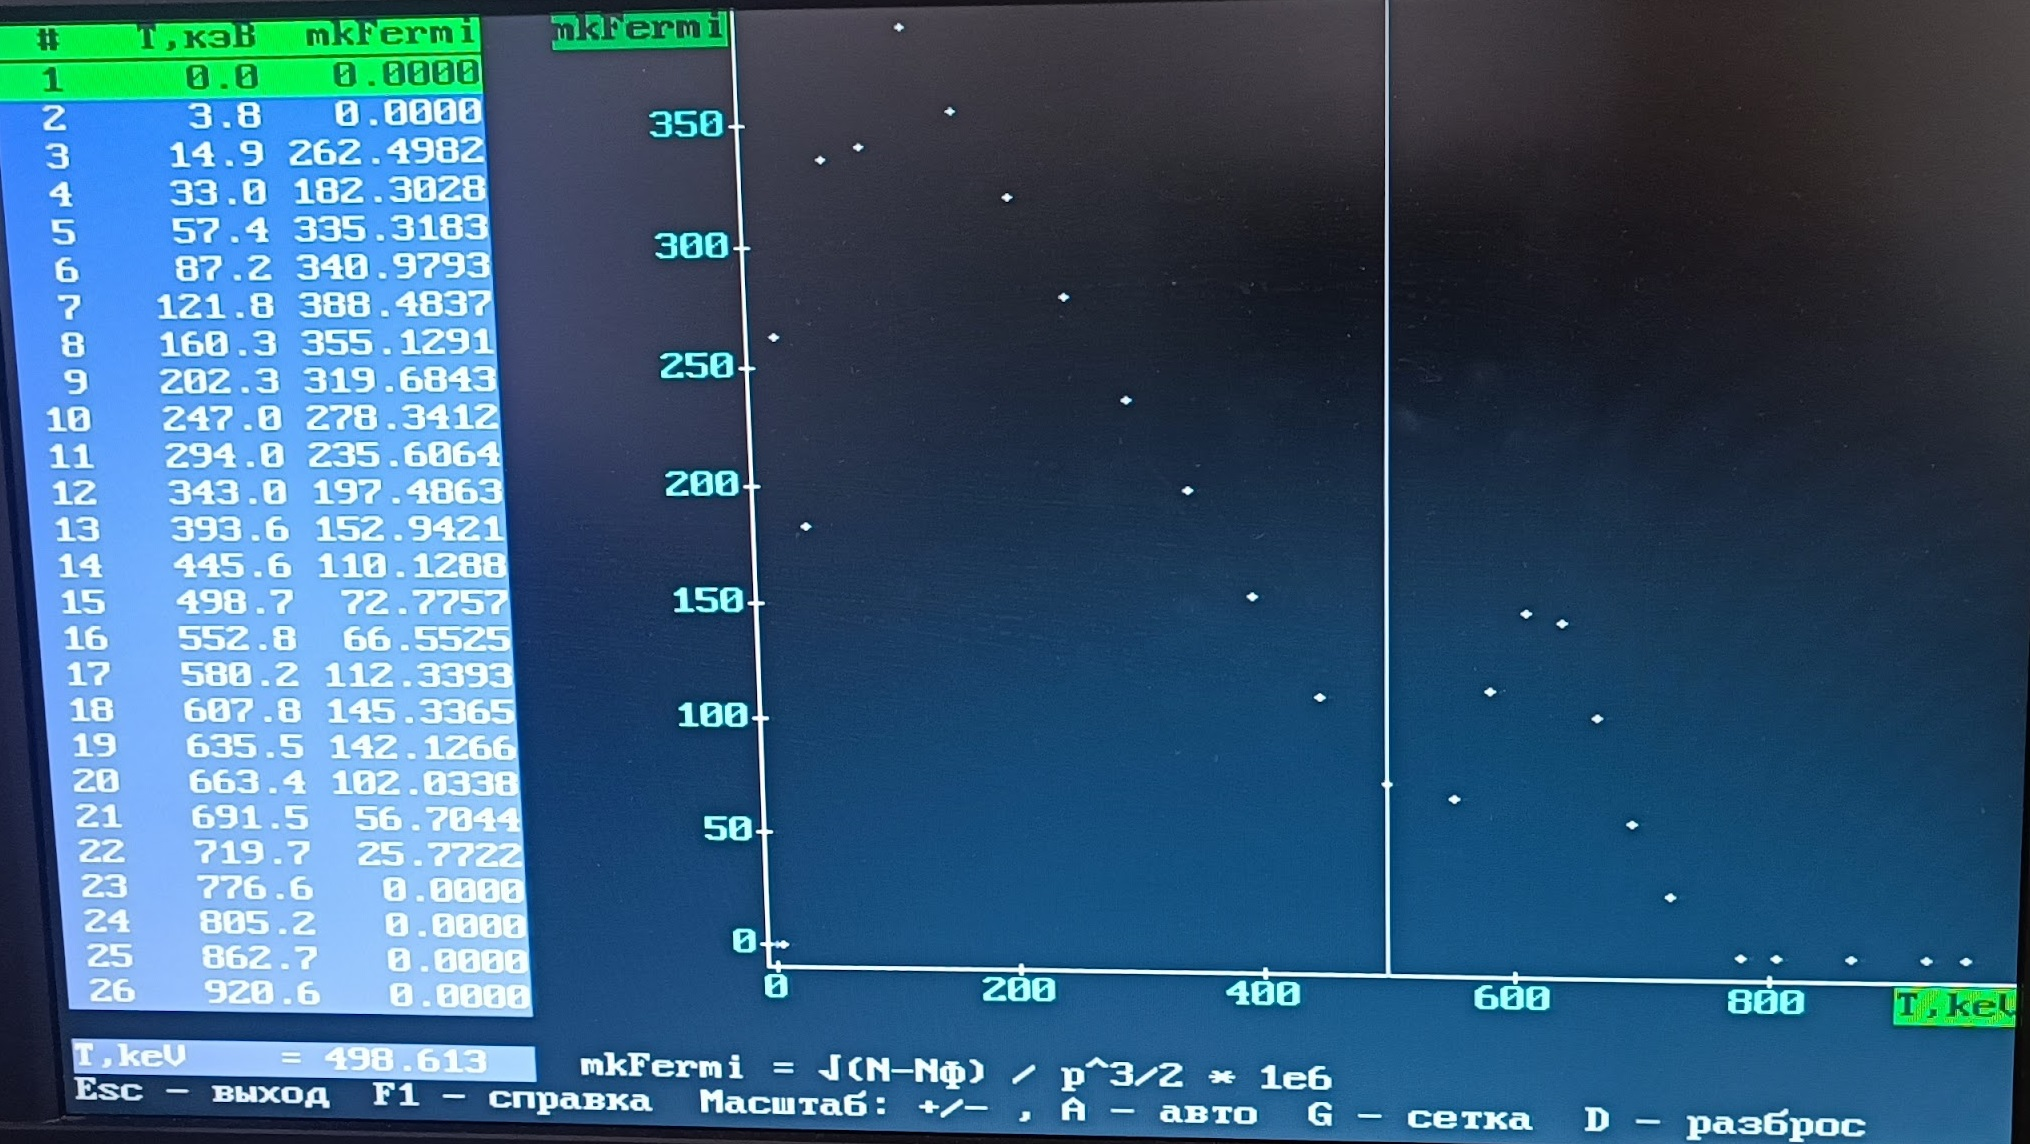
\includegraphics[width = 0.5\linewidth]{images/fermi_curie.jpg}
        \caption{График Ферми-Кюри}
        \label{fig:fermi-curie}
    \end{figure}
		
	Воспользовавшись графиком, получим, что $E_m \approx 600 \text{ кэВ}.$
    
    \section{Заключение}
    
    \begin{itemize}
       \item В ходе лабораторной работы с помощью магнитного спектрометра мы исследовали энергетический спектр $\beta$-частиц при распаде ядер $^{137}$Cs. Калибровку спектрометра осуществили по энергии электронов внутренней конверсии.
	
        \item Также мы определили максимальную энергию вылетающих электронов при $\beta$-распаде ядря $^{137}$Cs методом Ферми-Кюри: $E_m \approx 600$ кэВ.
    \end{itemize}
    
\end{document}